\section{Ambiente de referênciamento locais}
\begin{frame}{Ambiente de referênciamento locais}
\begin{block}{Variáveis locais estáticas}
	São vinculadas ao armazenamento antes da execução do programa e continuam até seu término.
	\begin{itemize}
	  \item + Endereçamento direto na memória.
	  \item + Não causam sobrecarga na alocação e desalocação.
	  \item - Não se comportam bem em programas recursivos.
	  \item - Representam um estado global.
	\end{itemize}
\end{block}
\end{frame}

\begin{frame}{Ambiente de referênciamento locais}
\begin{figure}[ht!]
 \centering
 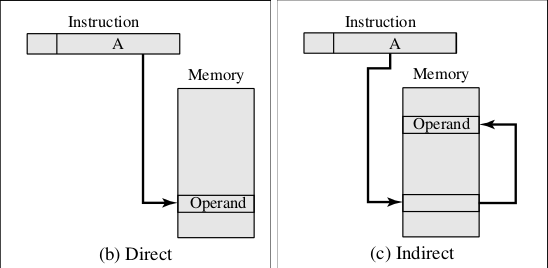
\includegraphics[scale=0.5]{./imgs/enderecamento.png}
\label{enderecamento}
\end{figure}
\end{frame}

\begin{frame}[fragile]{Ambiente de referênciamento locais}
\begin{lstlisting}
int sum (int arr[], int n)
{
    static int result = 0;
    if (n == 0)
        return result ;
    else {
        result += arr[n - 1];
        sum(arr, n - 1);
     }
}

int main(void) {
    int array[5] = {1,2,3,4,5};
    printf("%d\n", sum(array, 3));  // 6
    printf("%d\n", sum(array, 3));  // 12
    printf("%d\n", sum(array, 3));  // 18
    return 0;
}
\end{lstlisting}
\end{frame}

\begin{frame}{Ambiente de referênciamento locais}
\begin{block}{Variáveis locais dinâmicas na pilha}
	Variáveis dinâmicas na pilha, são vinculadas ao armazenamento quando o subprograma inicia sua execução e desvinculadas do armazenamento quando ele se encerra.
	\begin{itemize}
	  \item + Maior flexibilidade (programas recursivos).
	  \item - Sobrecarga na alocação e desalocação.
	  \item - Endereçamento indireto.
	\end{itemize}
\end{block}
\end{frame}

\begin{frame}{Ambiente de referênciamento locais}
\begin{block}{Exemplos}
	\begin{itemize}
	  \item ALGOL 60 e suas linguagens descendentes, possuem variáveis locais dinâmicas na pilha.
	  \item Funções em C possuem variáveis são dinâmicas na pilha a menos que sejam especificamente declaradas como static. 
	  \item Subprogramas Pascal e Ada e métodos em C++, Java, C\# têm somente variaveis dinâmicas na pilha. 
	\end{itemize}
\end{block}
\end{frame}

\section{Aninhamento de subprogramas} 
\begin{frame}[fragile]{Aninhamento de subprogramas}
Linguagens como ALGOL 68, Pascal e Ada, JavaScript, Python e Lua permitem aninhamento de subprogramas. Linguagens descententes de C não permitem aninhamento.
\begin{verbatim}
function hipotenusa(a, b) {
   function quadrado(x) {
      return x * x; 
   }
   return Math.sqrt(quadrado(a) + quadrado(b));
}
\end{verbatim}
\end{frame}